%cSpell:disable
\subsection{Wesentliche Begriffe}
\subsubsection{Beleihungsauslauf}
Der Beleihungsauslauf, auch als \ac{LtV} bekannt, ist eine zentrale Kennzahl in der Immobilienfinanzierung \parencite{BelWertV_3}. Er wird definiert als:
\begin{equation}
    \text{Beleihungsauslauf} = \frac{\text{Darlehensbetrag}}{\text{Beleihungswert}}
    \label{eq:ltv}
\end{equation}

\noindent wobei:
\begin{itemize}
    \item Der Darlehensbetrag ist die Höhe des Darlehens.
    \item Der Beleihungswert ist der langfristig erzielbare Wert einer Immobilie, unabhängig von kurzfristigen Marktschwankungen.
\end{itemize}

Ein niedrigerer Beleihungsauslauf signalisiert dem Kreditinstitut ein geringeres Ausfallrisiko. Ein höherer Beleihungsauslauf erhöht das Risiko und verschlechtert die Kreditbedingungen.

Zur Veranschaulichung wird ein Fallbeispiel einer Immobilienfinanzierung herangezogen. Dabei bewertet zunächst ein Gutachter ein Objekt, dessen Beleihungswert bei 500.000 Euro liegt. Ein Käufer beantragt einen Kredit von 275.000 Euro für den geplanten Hauskauf.
Der Beleihungsauslauf wird gemäß Gleichung \ref{eq:ltv} folgendermaßen berechnet:
\begin{equation}
    \text{Beleihungsauslauf} = \frac{\text{Darlehensbetrag}}{\text{Beleihungswert}} = \frac{275.000 \mbox{\texteuro}}{500.000 \mbox{\texteuro}} = 0,55 = 55\%
\end{equation}
Der Beleihungsauslauf in diesem Fall beträgt 55\%. Das bedeutet, dass 55\% des Immobilienwertes wird von der Bank finanziert. Die restlichen 45\% müssen durch Eigenkapital oder oder andere Einnahmequellen abgedeckt werden.
\subsubsection{Transitionsrisiken}
Transitionsrisiken bezeichnen finanzielle Risiken für Verluste, die im Zuge des Übergangs zu einer Wirtschaft mit weniger CO2-Emissionen und einer umweltfreundlicheren Ökonomie auftreten können \parencite{ecb2020climate}. Dies sind Risiken im Zusammenhang mit Technologie, Marktpreisen, Regulierung und Reputation

Der Bereich der Immobilien ist stark betroffen, da er für 40\% der weltweiten Treibhausgasemissionen verantwortlich ist \parencite{unepfi2023realestate}. Die neuen Gesetze zu Energiepreisen und CO2-Steuern verursachen die Hauptursachen dieser Risiken. Um die Wettbewerbsfähigkeit zu erhalten und Nachhaltigkeitsziele zu erreichen, sind Anpassungen unumgänglich.
\subsubsection{Physische Risiken}
Unter physischen Risiken versteht man Gefahren aus Naturereignissen mit negativen Folgen für Gesellschaft, Wirtschaft und Ökosysteme \parencite{greenvisionsolutions_transitorische_2024}. Diese Risiken werden in zwei Kategorien unterteilt. Akute Risiken entstehen durch plötzliche extreme Ereignisse wie Überschwemmungen oder Stürme. Chronische Risiken ergeben sich aus langfristigen klimatischen Veränderungen. Beispiele dafür sind der Meeresspiegelanstieg, Wasserstress, Biodiversitätsverlust und Mangel an Ressourcen.\parencite{dnb2019values}.

\subsubsection{Klimaszenarien des NGFS}
Das \ac{NGFS} hat 72 verschiedene Klimaszenarien entwickelt, wovon sechs für diese Arbeit ausgewählt wurden. Diese sechs Szenarien repräsentieren ein breites Spektrum möglicher Entwicklungen unter Berücksichtigung verschiedener physischer Risiken und Transitionsrisiken \parencite{NGFS2021}. In Abbildung \ref{fig:ngfs} ist die Darstellung der sechs Haupt-Szenarien des NGFS im Rahmenwerk zu sehen. In Tabelle \ref{tab:ngfs-framework} sind ausführliche Erläuterungen zu diesen Situationen enthalten.

\begin{figure}[htbp]
    \centering
    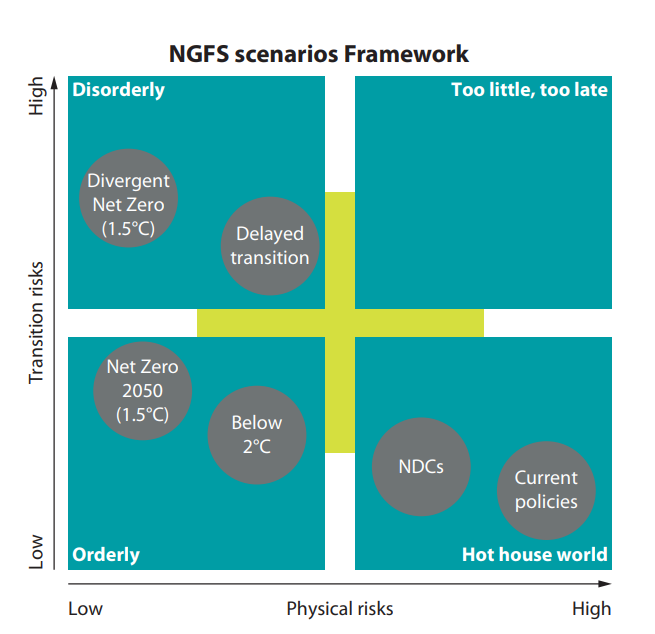
\includegraphics[width=0.8\textwidth]{figures/NGFS.png}
    \caption{NGFS Klimaszenario-Framework. Quelle: NGFS Climate Scenarios for central banks and supervisors (June 2021)}
    \label{fig:ngfs}
\end{figure}
\FloatBarrier

\begin{table}[htbp]
    \centering
    \small
    \caption{Überblick über NGFS-Rahmen zur Klassifizierung von Klimarisiken. In Anlehnung an Quelle: NGFS Climate Scenarios for central banks and supervisors (June 2021).}
    \label{tab:ngfs-framework}
    \begin{tabularx}{1.0\textwidth}{>{\raggedright\arraybackslash}X >{\centering\arraybackslash}X >{\centering\arraybackslash}X >{\raggedright\arraybackslash}X}
        \toprule
        \textbf{Szenario} & \textbf{Transitionsrisiken} & \textbf{Physische Risiken} & \textbf{Beschreibung} \\
        \midrule
        Orderly & Niedrig & Niedrig & Maßnahmen zur Klimapolitik werden frühzeitig eingeführt und schrittweise verschärft. Sowohl Transitions- als auch physische Risiken bleiben gering. \\
        \addlinespace
        Disorderly & Hoch & Niedrig & Höhere Transitionsrisiken aufgrund verzögerter oder inkonsistenter Klimapolitiken \\
        \addlinespace
        Hot house world & Niedrig & Hoch & Begrenzte Klimapolitik in einigen Ländern; globale Bemühungen unzureichend gegen Erwärmung. Folge: Schwere physische Risiken mit irreversiblen Auswirkungen wie Meeresspiegelanstieg.\\
        \addlinespace
        Too little, too late & Hoch & Hoch & Extremste Szenarien. Unzureichende Maßnahmen führen zu Katastrophen und erzwingen einen ungeordneten Übergang. \\
        \bottomrule
    \end{tabularx}
\end{table}
\FloatBarrier

Die Szenarien "`Orderly"', "`Disorderly"' und "`Hot House World"' für die Jahre 2030, 2040 und 2050 stehen im Mittelpunkt. Im EZB-Klimarisiko-Stresstest werden sie mittels eines Bottom-up-Ansatzes berücksichtigt und beinhalten sowohl Transitions- als auch physische
Risiken \parencite{ECB2022ClimateStressTest}. Diese Szenarien bilden die Grundlage für die Analyse der potenziellen Auswirkungen verschiedener Klimapolitiken auf den Immobiliensektor über einen längeren Zeitraum und ermöglichen eine detaillierte Untersuchung der Bruttowertschöpfung in diesem Sektor.

\subsubsection{Abflussmenge bei Hochwasser}\label{sec:HQ}

Die Festlegung von Hochwasserrisikogebieten in Deutschland erfolgt gesetzlich anhand der Anzahl von HQ\textsubscript{T\textsubscript{n} }-Ereignissen gemäß dem \textcite{WHG73}. Hierbei steht HQ für die Abflussmenge bei Hochwasser, während T\textsubscript{n} für den statistische Wiederkehrperiode des Ereignisses. Beispielsweise bezeichnet ein HQ\textsubscript{100} ein statistisch einmal in 100 Jahren auftretendes Hochwasserereignis.
In Bayern erfolgt eine detailliertere Klassifizierung von Hochwasserereignissen anhand ihrer statistischen Häufigkeit \autocite{BayLfU2019}:
\begin{itemize}
\item HQ\textsubscript{häufig}: Ein Hochwasser, das im Mittel alle 5 bis 20 Jahre auftritt und als "häufiges Hochwasser" bezeichnet wird.
\item HQ\textsubscript{100}: Ein Ereignis, das statistisch einmal in 100 Jahren zu erwarten ist.
\item HQ\textsubscript{extrem}: Ein sehr seltenes Extremhochwasser, das zu deutlich höheren Wasserständen als ein HQ\textsubscript{100} führen kann.
\end{itemize}
Durch diese Einteilung ist es möglich, Hochwassergefahren genauer zu bewerten und die Entwicklung von Schutzmaßnahmen zu unterstützen.

\subsubsection{Energieeffizienzklasse}

Der Energieeffizienzklassen, auch \ac{EPC} bekannt, ist eine zentrale Kennzahl in der Immobilien. Sie bewertet, wie viel Energie ein Gebäude verbraucht. Es gibt Klassen von A+ bis H, wobei A+ am besten und H am schlechtesten ist. Diese Einteilung zeigt, wie energiesparend ein Haus oder eine Wohnung ist. Das ist wichtig für Hausbesitzer, Mieter und Käufer. Mit dieser Information können sie besser entscheiden, wie viel Energie ein Gebäude braucht.
Die Klassifizierung für Energieeffizienzklassen  erfolgt anhand der Effizienz, die in kWh pro m² gemessen wird \parencite{gebaeudeenergiegesetz2020}. Dabei dient die Nutzfläche als Grundlage, welche meist etwas größer als die Wohfläche ist. Aus Tabelle \ref{tab:epc} ergeben sich folgende Grenzwerte für die Klassen.
\begin{table}[htbp]
    \centering
    \caption{Überblick über Energieeffizienzklassen für Gebäude. Quelle:Gebäudeenergiegesetz (2020)}
    \label{tab:epc}
    \begin{tabularx}{\textwidth}{>{\raggedright\arraybackslash}X >{\raggedright\arraybackslash}X}
        \toprule
        \textbf{Energieverbrauch (kWh/m²a)} & \textbf{Energielabel} \\
        \midrule
        $\leq$ 30 & A+ \\
        30 -- 50 & A \\
        50 -- 75 & B \\
        75 -- 100 & C \\
        100 -- 130 & D \\
        130 -- 160 & E \\
        160 -- 200 & F \\
        200 -- 250 & G \\
        $\geq$ 250 & H \\
        \bottomrule
    \end{tabularx}
\end{table}